\documentclass[10pt,a4paper,titlepage]{report}
\usepackage[utf8]{inputenc}
\usepackage{amsmath}
\usepackage{amsfonts}
\usepackage{amssymb}
\usepackage{graphicx}
\usepackage{xcolor}
\usepackage{minted}

\newcommand{\HRule}[1]{\rule{\linewidth}{#1}}

\nonstopmode


\begin{document}
{\fontfamily{cmr}\selectfont
\title{ \normalsize \textsc{}
\\ [2.0cm]
\HRule{0.5pt} \\
\LARGE \textbf{\uppercase{Aggregate Functions}
\HRule{2pt} \\ [0.5cm]
\normalsize \today \vspace*{5\baselineskip}}
}

\date{}

\author{
	Rwithik Manoj \\
	College of Engineering, Trivandrum \\
	Department of Computer Science and Engineering }

\maketitle
\newpage

\sectionfont{\scshape}

\begin{enumerate}
	\item Find the class average for the subject ‘Physics’\newline
		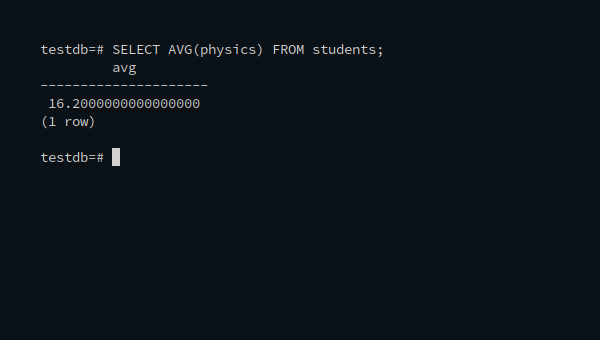
\includegraphics[width=\linewidth]{../Images/Aggregate/1.png}\newline
\item Find the highest marks for mathematics (To be displayed as highest\_marks\_maths).\newline
		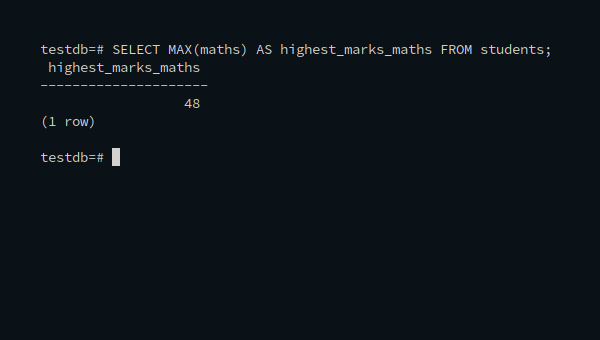
\includegraphics[width=\linewidth]{../Images/Aggregate/2.png}\newline
\item Find the lowest marks for chemistry(To be displayed as lowest\_mark\_chemistry)\newline
		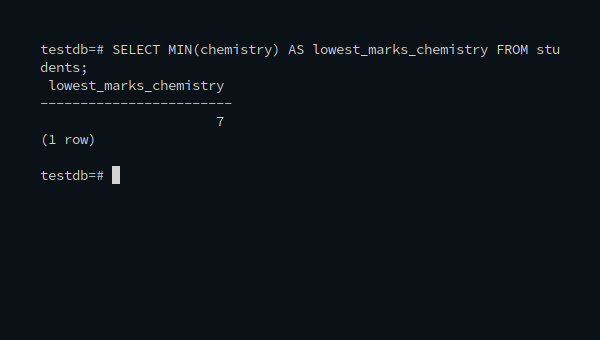
\includegraphics[width=\linewidth]{../Images/Aggregate/3.png}\newline
	\item Find the total number of students who has got a ‘pass’ in physics.\newline
		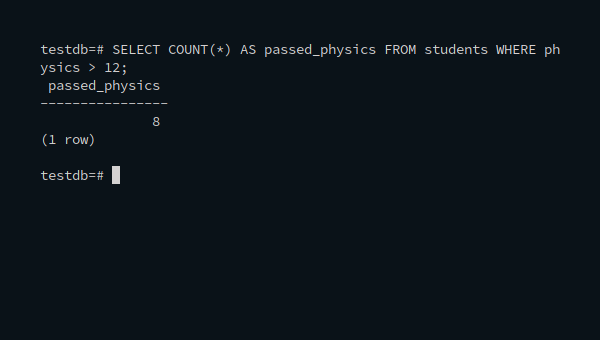
\includegraphics[width=\linewidth]{../Images/Aggregate/4.png}\newline
	\item Generate the list of students who have passed in all the subjects\newline
		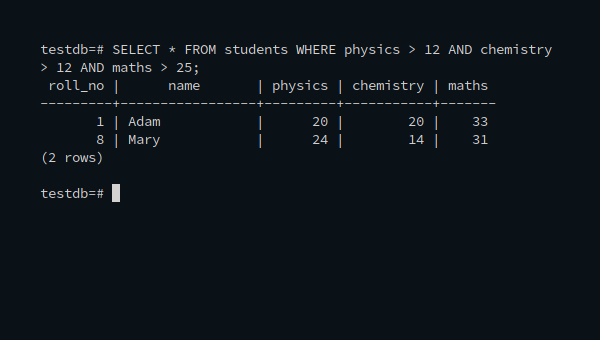
\includegraphics[width=\linewidth]{../Images/Aggregate/5.png}\newline
	\item Generate a rank list for the class.Indicate Pass/Fail. Ranking based on total marks obtained by the
			students.\newline
		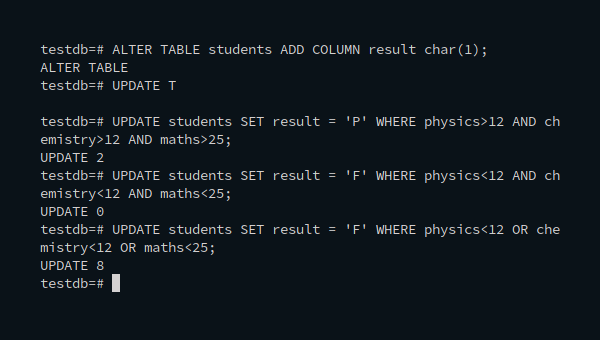
\includegraphics[width=\linewidth]{../Images/Aggregate/6.png}\newline
		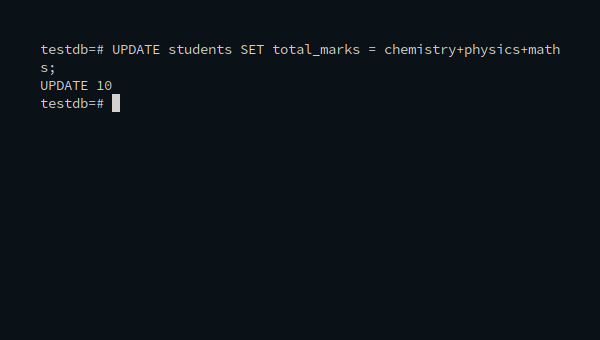
\includegraphics[width=\linewidth]{../Images/Aggregate/7.png}\newline
		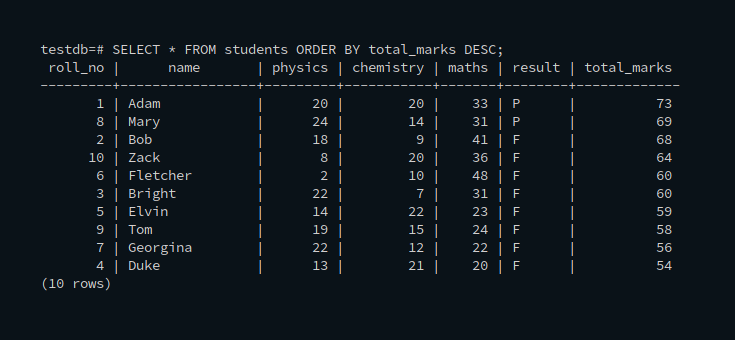
\includegraphics[width=\linewidth]{../Images/Aggregate/8.png}\newline
	\item Find pass percentage of the class for mathematics.\newline
		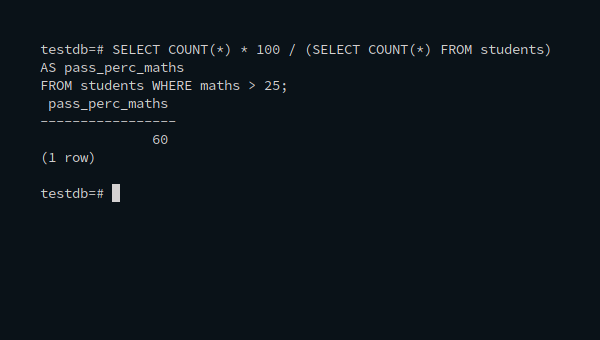
\includegraphics[width=\linewidth]{../Images/Aggregate/10.png}\newline
	\item Find the overall pass percentage for all class.\newline
		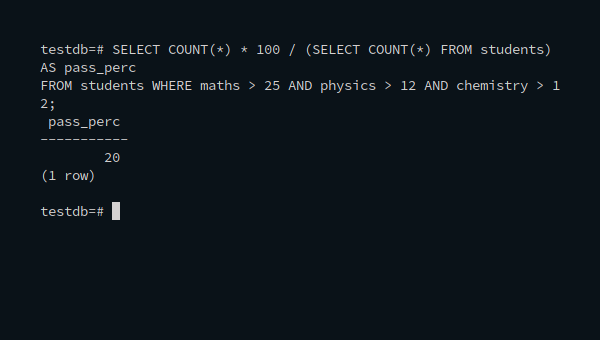
\includegraphics[width=\linewidth]{../Images/Aggregate/11.png}\newline
	\item Find the class average.\newline
		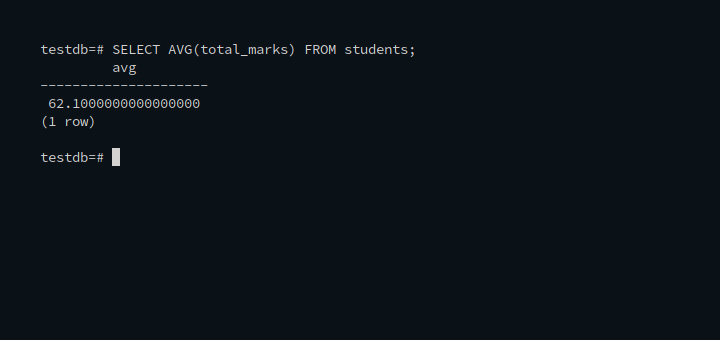
\includegraphics[width=\linewidth]{../Images/Aggregate/12.png}\newline
	\item Find the total number of students who have got a Pass.\newline
		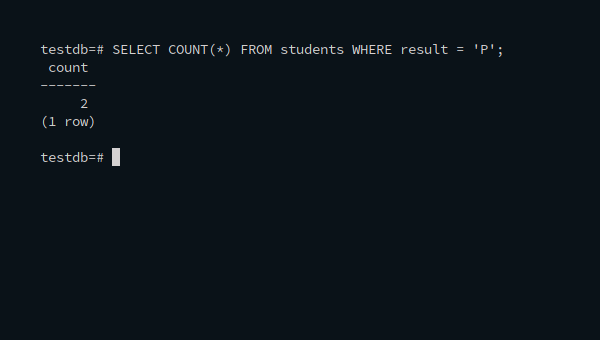
\includegraphics[width=\linewidth]{../Images/Aggregate/13.png}\newline
\end{enumerate}

\subsubsection{RESULT}

The query was executed successfully and output was obtained.

}
\end{document}
